\chapter{Complex Circuits with OpAmps}
\section{Ideal Half-Wave Rectifier}

\begin{figure}
	\centering
	\begin{subfigure}{0.4\textwidth}
		\centering
		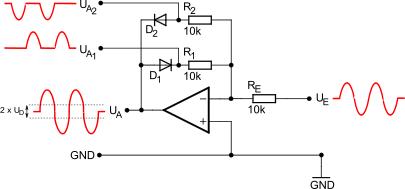
\includegraphics[width=.9\linewidth]{./img/schem-rectifier.pdf}
		\caption{Ideal Rectifier}
		\label{schem:rectifier}
	\end{subfigure}
	\begin{subfigure}{0.4\textwidth}
		\centering
		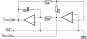
\includegraphics[width=.9\linewidth]{./img/schem-wavegen.pdf}
		\caption{Square and Triangle Wave Generator}
		\label{schem:wavegen}
	\end{subfigure}
	\caption{}
\end{figure}

A basic half-wave rectifier consists of a diode a resistor to provide a load to the diode.
All diodes carry an inherent voltage drop, so the signal level is lowered by \SI{0.2}{\volt} (Schottky diode) to \SI{0.7}{\volt} (silicon diode).
To combat this amplitude loss, an ideal rectifier is used.

An ideal rectifier (\autoref{schem:rectifier}) uses an operational amplifier with separate feedback paths for the positive and negative half wave.
Looking just at the output of the opamp, the two diodes in the feedback path are essentially anti-parallel, the rest forming an inverting ampifier with gain 1.
As the voltage drop due to the diodes in the feedback path is compensated by the feedback loop, the output of the opamp follows the input, with the amplitude increased by one diode drop.
This means that at zero crossings, in theory the output voltage is discontinuous, introducing high frequency components that may lead to undesired effects.

To now recover the rectified (or more specifically separated) positive and negative half waves, the circuit is tapped in the middle of each feedback line, where the output signal amplitude matches the input signal amplitude (this can be verified by looking at the two identical resistors connected to the inverting input, carrying the same current, they have an equal voltage across them with the inverting input being a virtual ground).

\section{Square and Triangle Wave Generator}

Operational amplifiers can also be operated with positive feedback.
As any signal is fed back to the input in phase, the output voltage is limited only by the rail voltage of the opamp, and will not remain stable between the rails.

\section{Programmable Differential Equation}
